%----------------------------------------------------------------------------
%----------------------------------------------------------------------------
%				    	SETUP
%----------------------------------------------------------------------------
%----------------------------------------------------------------------------

\documentclass[11pt]{article}

%----------------------------------------------------------------------------
%			  	   PACKAGES
%----------------------------------------------------------------------------

%%%%%%%%%%%%%%%%%%%%%%%
% 	  Packages
%%%%%%%%%%%%%%%%%%%%%%%

%% Fonts and Symbols
%% --------------------------
\usepackage{
	amsmath,			% math operators
	amssymb,			% math symbols
	courier,			% better tt font for listings
	soul,				% strike through with \st{}
	url,				% embed urls in text
	xcolor,				% color!
	xfrac,				% fancy fractions
}

% preserve default font for URLs
\renewcommand*{\UrlFont}{\rmfamily}		

%% Graphics
%% --------------------
\usepackage{
	graphicx,			% allows insertion of images
	subfigure,			% allows subfigures (a), (b), etc.
}				
\graphicspath{ {graphics/} }	% (graphicx) relative path to graphics folder				

%% Tables
%% --------------------------
\usepackage{
	booktabs,			% better tables, discourages vertical rulings
	multicol,			% allow multi columns
}

%% Layout Alteration
%% --------------------------
\usepackage{			
%	caption,			% line breaks in captions with \\
%	changepage,			% change margins for PARTS of pages with (adjustwidth)
	geometry,			% change the margins for specific PAGES
	parskip,			% disable indents
	rotating,			% sideways figures
	setspace,			% single, double spacing
}
\geometry{				% specify page size options for (geometry)
	a4paper, 			% paper size
	hmargin=1in,		% horizontal margins
	vmargin=1in,		% vertical margins
}	


%% Units
%% --------------------------
\usepackage{
	siunitx,			% has S (decimal align) column type
}
\sisetup{input-symbols = {()},  % do not treat "(" and ")" in any special way
	group-digits  = false, 	% no grouping of digits
%	load-configurations = abbreviations,
%	per-mode = symbol,
}

%% Misc
%% --------------------------
\usepackage{
	enumitem,			% better control of enumerations, descriptions, etc
%	listings,			% source code import and display
	todonotes,			% \todo[inline]{stuff} and \missingfigure{descr}
}

%% References
%% --------------------------
\usepackage[backend=biber,style=ieee]{biblatex}
\addbibresource{ELEC340_Lab_03.bib}

%----------------------------------------------------------------------------
%		     MACROS AND COMMANDS
%----------------------------------------------------------------------------

% Defines a new command for the horizontal lines, change thickness here
\newcommand{\HRule}{\rule{\linewidth}{0.5mm}} 

% override S column type with centered text column
\newcommand{\textcol}[1]{\multicolumn{1}{c}{#1}}

% awkward capitalization
\newcommand{\mefisto}{MEFiSTo}

%----------------------------------------------------------------------------
%----------------------------------------------------------------------------
%				   DOCUMENT
%----------------------------------------------------------------------------
%----------------------------------------------------------------------------

\begin{document}

\begin{titlepage}

\center
 
% Header
\textsc{\LARGE University of Victoria}\\[1cm] 	% Name of your university/college
\textsc{\Large ELEC 340}\\[0.5cm] 			% Major heading such as course name
\textsc{\large Applied Electromagnetics and Photonics}\\[0.5cm] 		% Minor heading such as course title


% Lab Title
\HRule \\[0.4cm]
{\huge \bfseries Lab 1 - Time-Varying Electromagnetic Fields}\\[0.2cm] % Title of your document
\HRule \\[1.5cm]
 
 
%Lab Instructor Details
\begin{minipage}{0.7\textwidth}
\begin{flushleft} 

\large\emph{Instructor:} \\
Dr. Poman \textsc{So} \\
\vspace{12 pt}
% I don't know the name of our TA :(
%\emph{Teaching Assistant:} \\ 
%Grace \textsc{Hui}

\end{flushleft}
\end{minipage}
~
\begin{minipage}{0.1\textwidth}
\begin{flushright} \large

\vspace{12 pt}

\end{flushright}
\end{minipage}\\[2cm]


% Lab members
\Large A.K. \textsc{Blanken}
\large V00809798 \\
\Large T. \textsc{Stephen}
\large V00812021	\\
A01 - B03\\[1.5cm] 


{\large 3 February, 2016}\\ % Date

\begin{figure}[b]
	\centering
	\includegraphics[scale=0.3]{UVic_logo}
\end{figure}

\end{titlepage}


\doublespacing
\section{Objective}\label{sec:objective}
This experiment will use a \mefisto{} simulation to investigate the propagation of an electromagnetic wave through a waveguide.
The results of the simulation will validate the Helmholtz equation and provide insight into the propagation properties of plane waves.

\section{Introduction}\label{sec:intro}
Faraday's and Ampere's Laws can be applied \cite[pp. 15-16]{lab-manual} to a medium with constant permittivity and permeability to yeild the Helmholtz equation:
\begin{equation}
	\del^2 \phasor{E} = - \omega^2 \mu \epsilon \phasor{E} = \gamma^2 \phasor{E}.
\end{equation}
This relation implies that \emph{something...}

\textit{More about intrinsic impedance effect on propagation.}

\textit{A little bit about polarization.}

\section{Procedure}\label{sec:procedure}
\subsection{Uniform plane waves in a parallel plate structure}\label{sec:upw}
A perfect parallel plate wave guide is created in \mefisto{} by bounding a region of air with opposite, perfect electrical and magnetic boundaries.
The ends of the waveguide are covered with an absorbing boundary.
A wave source fills a vertical slice of the waveguide and will act on the transverse and parallel animation regions.
This arrangement is shown in Fig. \ref{fig:waveguide}, with the bottom electrical boundary, animation regions and source present.

\begin{figure}[tbph]
	\centering
	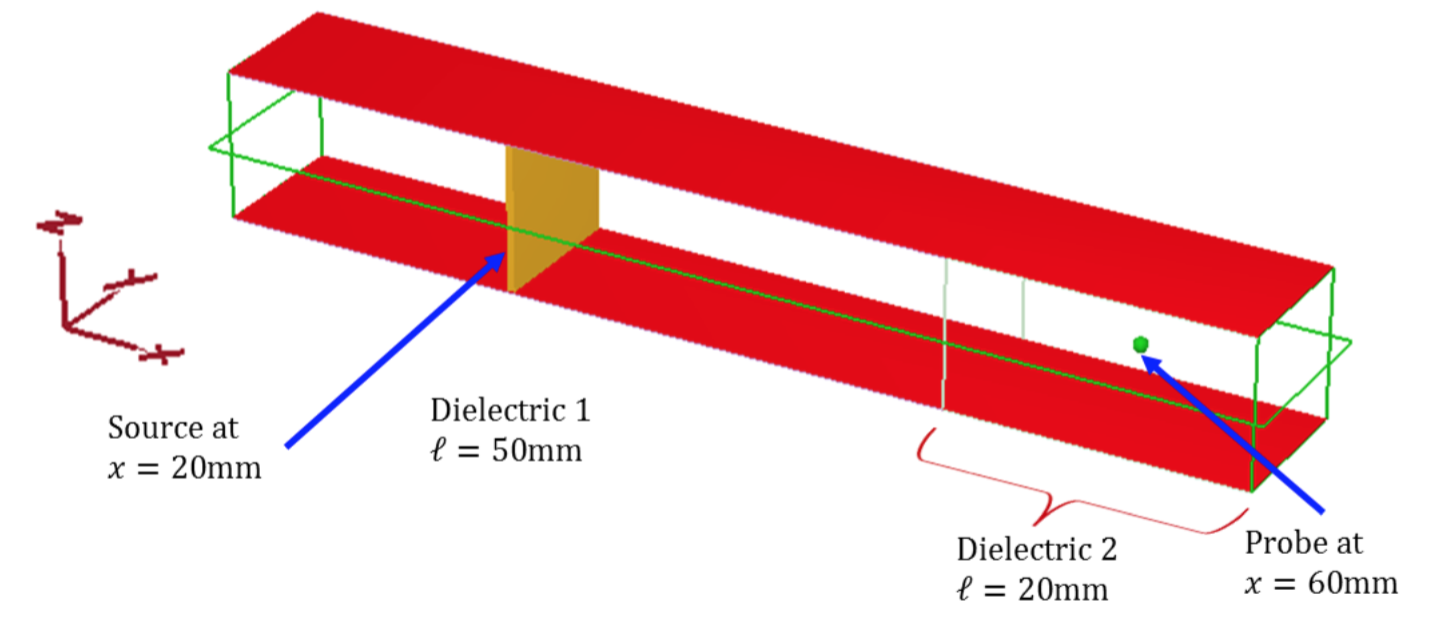
\includegraphics[width=0.7\linewidth]{graphics/waveguide}
	\caption{Perfect waveguide with dimensions 60 mm \by 10 mm \by 10 mm}
	\label{fig:waveguide}
\end{figure}

The source emits a wave with $f = \SI{15}{\giga\hertz}$ that travels through the medium, bounded by the walls of the waveguide.
The solid red color of the $yz$-animation plane in Fig. \ref{fig:Task1-2dsurface} shows that the wave travels as a plane wave from its origin through the waveguide.

\begin{figure}[tbph]
	\centering
	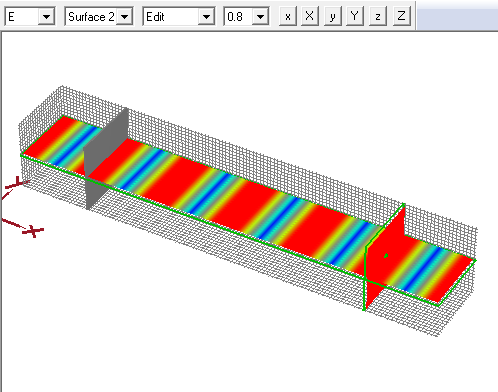
\includegraphics[width=0.7\linewidth]{graphics/Task1-2dsurface}
	\caption{Wave propagation in air-filled waveguide}
	\label{fig:Task1-2dsurface}
\end{figure}

The wave that is emitted from the source looks like a plane wave when we look at the small portion of it that is displayed in the y-z animation region.
The solid red colour indicates an infinite plane wave.
This agrees with the theory that a spherical wave can be approximated as a plane wave in the far field region as well as when looking at only a small portion of the wave. 

The physical properties of the propagation medium can be determined by examining the wave structure from Fig. \ref{fig:Task1-2dsurface}

\begin{figure}[tbph]
	\centering
	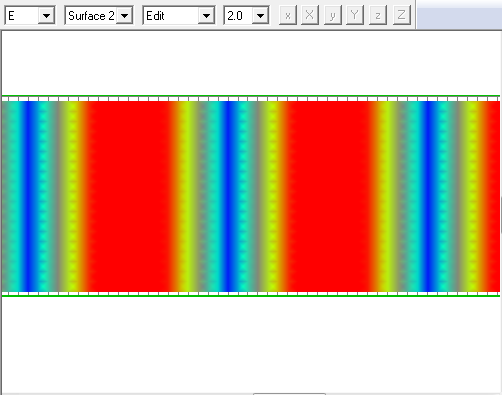
\includegraphics[width=0.7\linewidth]{graphics/Task1-scale}
	\caption{$xy$ view of propagation in Fig. \ref{fig:Task1-2dsurface}, with 0.5 mm mesh}
	\label{fig:Task1-scale}
\end{figure}

With this color scheme, blue regions indicate minima and maxima of the wave.
There are 20 grid square between adjacent blue regions in Fig. \ref{fig:Task1-scale}, corresponding the distance between a peak and trough.
At 0.5 mm mesh resolution, this indicates that $\lambda = \SI{20}{\milli\meter}$.

\newpage
\subsection{Waves in a non-ideal parallel plate structure}\label{sec:non-ideal}
Removing the magnetic sidewalls from the waveguide allows the wave energy to escape the confines of the guide.
When this change is made the wave propagation appears spherical near the source.
As the energy moves away from the source, the propagation becomes more planar.
This can be seen in Fig. \ref{fig:non-ideal}\subref{fig:3d}.
Fig. \ref{fig:non-ideal}\subref{fig:yz} shows that the orientation of all $\vec{E_z}$ are identical but their magnitude is not.

\begin{figure}[htpb]
	\centering
	\subfigure[]
	{
		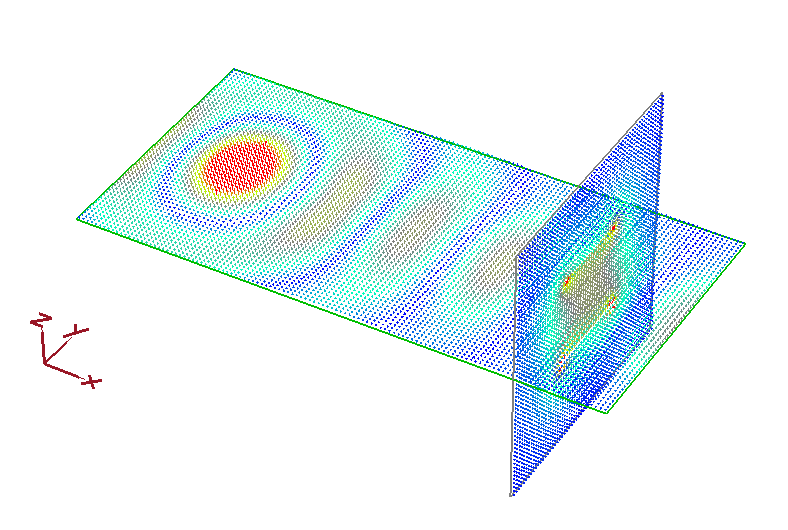
\includegraphics[width=0.575\linewidth]{graphics/Task2-3d-animation}
		\label{fig:3d}
	}
	\subfigure[$yz$-orientation]
	{
		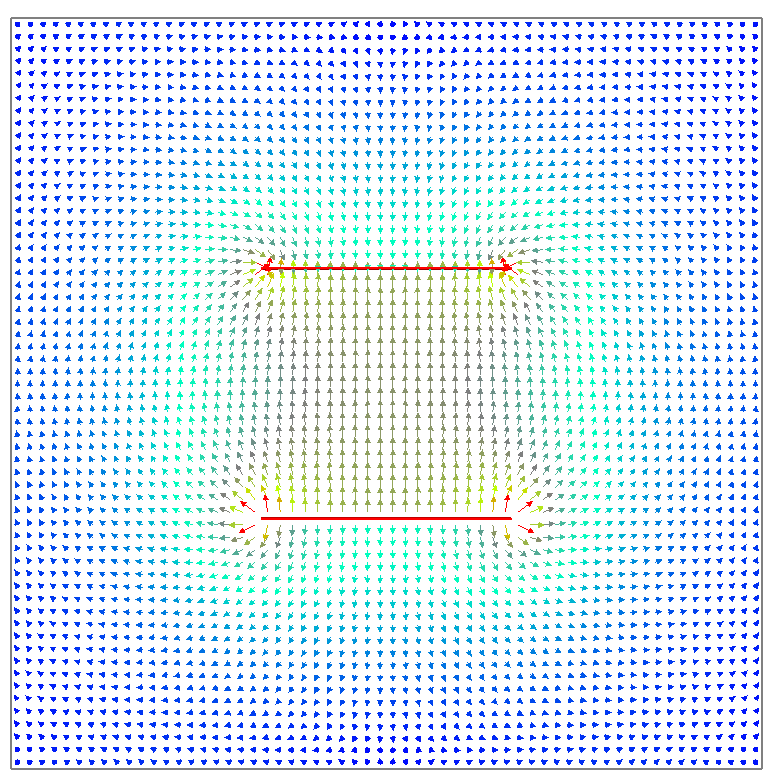
\includegraphics[width=0.375\linewidth]{graphics/Task2-yz-animation}
		\label{fig:yz}
	}
	\caption{Propagation in a non-ideal parallel plate}
	\label{fig:non-ideal}
\end{figure} 

\subsection{Dielectric and lossy media}\label{sec:dielectric}
The narrow-wide arrangement from Section \ref{sec:non-ideal} is changed to include a lossy dielectric between the top and bottom electric boundaries.
The boundaries with dielectric are shown in Fig. \ref{fig:plate-with-es}.

\begin{figure}[tbph]
	\centering
	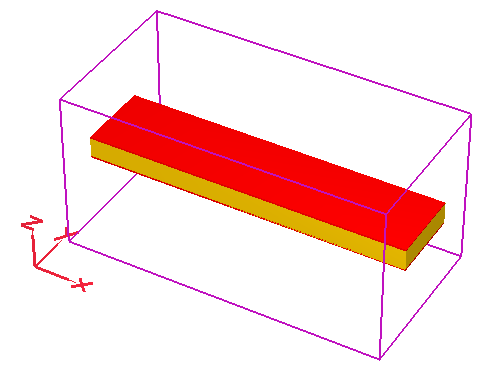
\includegraphics[width=0.7\linewidth]{graphics/plate-with-es}
	\caption{Waveguide containing a lossy dielectric material}
	\label{fig:plate-with-es}
\end{figure}

Propagation in the dielectric is shown in Fig. \ref{fig:Task3-3d-animation}.

\begin{figure}[tbph]
	\centering
	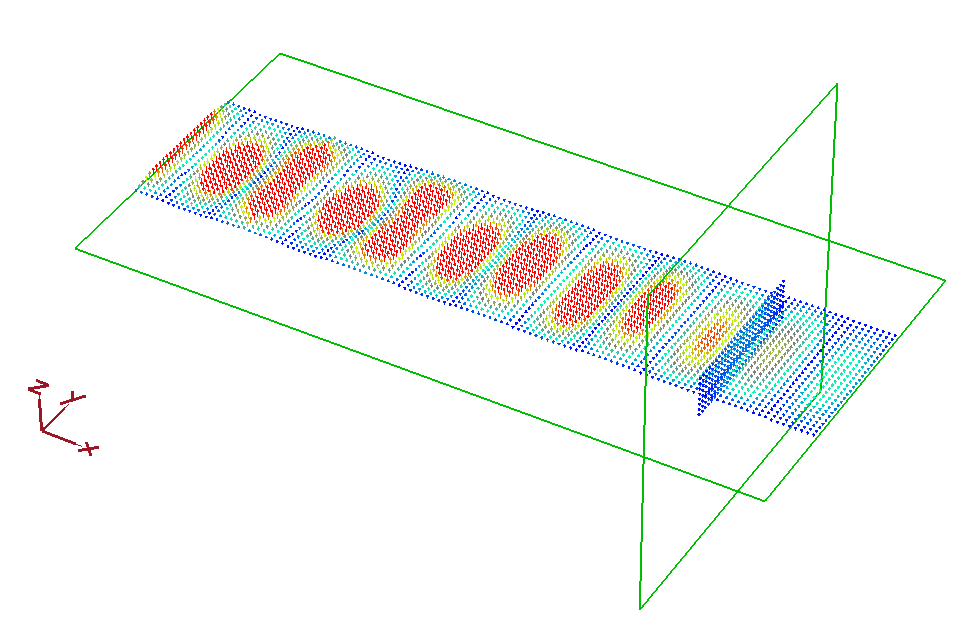
\includegraphics[width=0.7\linewidth]{graphics/Task3-3d-animation}
	\caption{Propagation in a waveguide filled with a dielectric where $\epsilon_r = 4$ and $\sigma = 0.5$}
	\label{fig:Task3-3d-animation}
\end{figure}

The wave attenuates as it travels through the waveguide as a result of $\sigma > 0$.

\section{Discussion}\label{sec:discussion}
\paragraph{Task 4} \textit{Compare the phase velocity to what you found in Section \ref{sec:upw}.}

By recording the distance traveled by a wave peak in one step of the animation, we found that:
\begin{equation*}
	u_{ph} = {\Delta x \over \Delta t} = {\SI{0.5}{\milli\meter} \over \SI{0.166}{\pico\second}} = \SI{3.01E8}{\meter\per\second}.
\end{equation*}
We found that $\lambda = \SI{20}{\milli\meter}$ in Section \ref{sec:upw} which implies that $u_{ph} = c_0$. The discrepancy between the two numbers is likely the result of a rounding error in \mefisto.

\paragraph{Task 7} \textit{Reduce the plate spacing to 4 mm and increase the width to 14 mm in the environment used for Section \ref{sec:non-ideal}.
Does the far field in the $xy$ and $yz$ planes behave like a uniform plane wave?}

Narrowing the gap between the electric field boundaries and widening them creates the propagation patterns shown in Fig. \ref{fig:narrow}.

\begin{figure}[htpb]
	\centering
	\subfigure[]
	{
		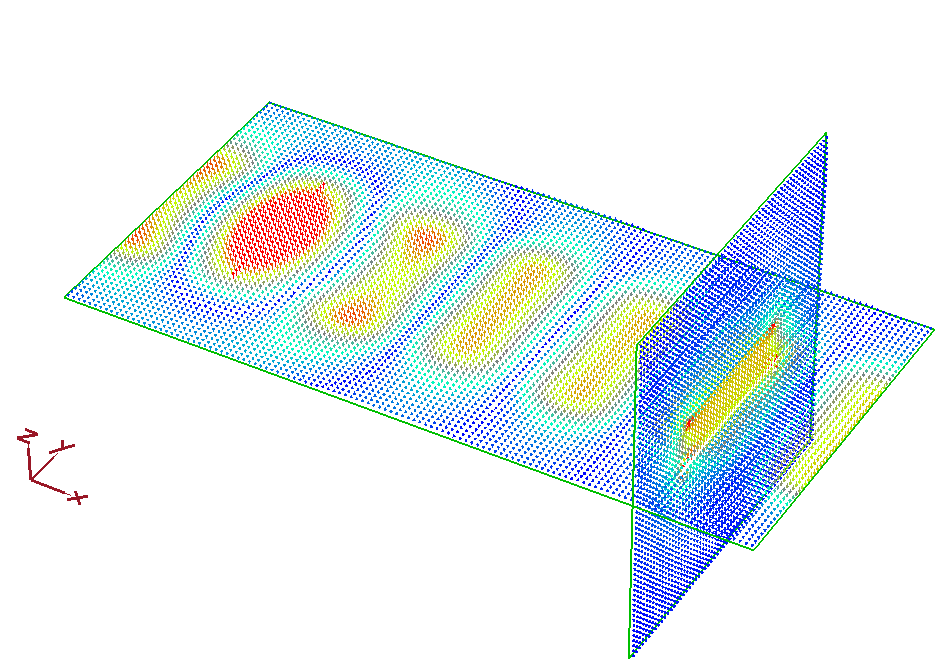
\includegraphics[width=0.575\linewidth]{graphics/Task2-3d-narrowplate}
		\label{fig:3d-narrow}
	}
	\subfigure[$yz$-orientation]
	{
		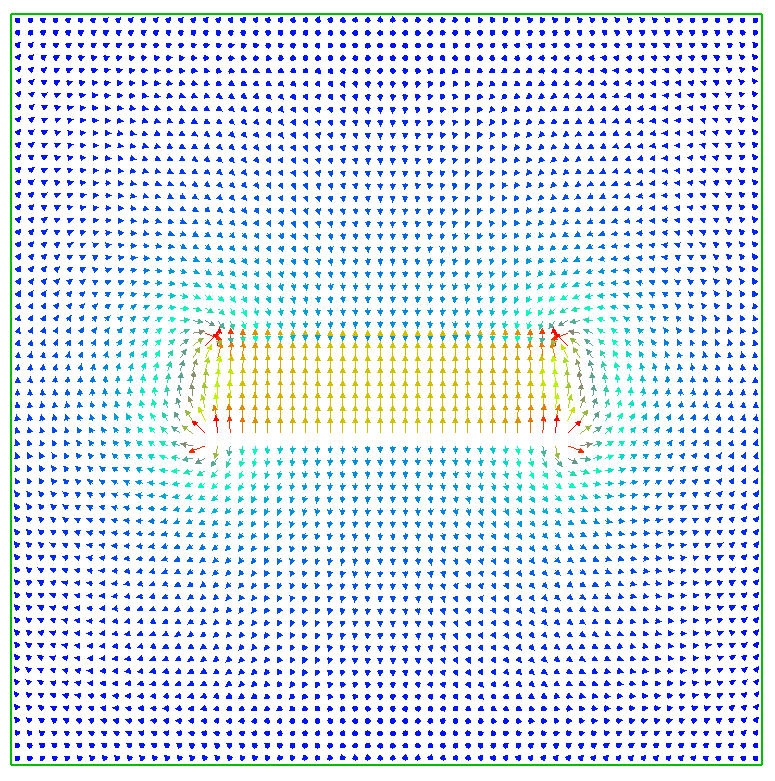
\includegraphics[width=0.375\linewidth]{graphics/Task2-yz-narrowplate}
		\label{fig:yz-narrow}
	}
	\caption{Propagation in a non-ideal, narrow parallel plate}
	\label{fig:narrow}
\end{figure}

The magnitude of the waves in Fig. \ref{fig:narrow}\subref{fig:3d-narrow} is greater than those in Fig. \ref{fig:non-ideal}\subref{fig:3d} and the groups have a much shorter and wider region of similar magnitude.
Fig. \ref{fig:narrow}\subref{fig:yz-narrow} confirms that both the direction and magnitude of the wave are similar far from the source.
Changing the electric field arrangement to make the separation smaller and boundaries wider has restored the plane wave behavior for the region between the boundaries.

\paragraph{Task 8} \textit{Determine $\alpha$ and $\beta$ for the waveguide with dielectric from Section \ref{sec:dielectric}.}

The lab manual suggests using Fig. \ref{fig:Task3-mesh} to determine the attenuation of the wave with equations \eqref{eqn:alpha} and \eqref{eqn:beta}.

\begin{figure}[tbph]
	\centering
	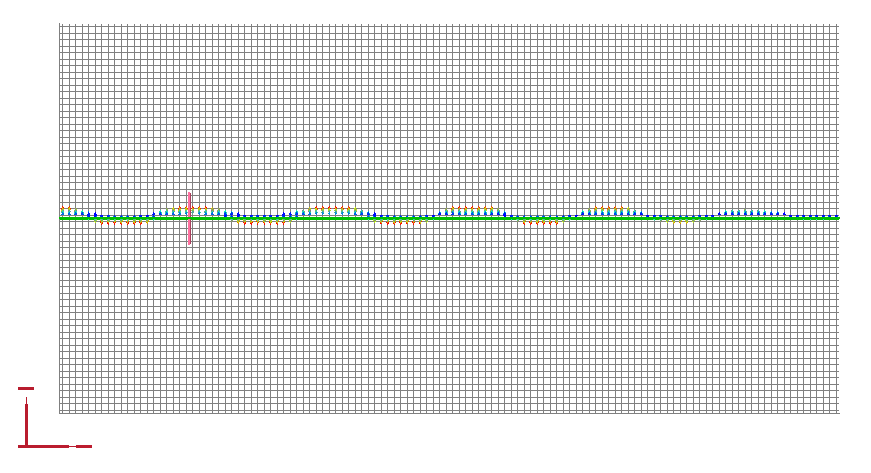
\includegraphics[width=0.7\linewidth]{graphics/Task3-mesh}
	\caption{$xz$ view of Fig. \ref{fig:Task3-3d-animation}}
	\label{fig:Task3-mesh}
\end{figure}
\begin{align}
	\alpha &= { \ln \left( { E_z(x_1) \over E_z(x_2) } \right) \over m \Delta x } \label{eqn:alpha} \\
	\beta &= { 2 \pi \over \lambda } \label{eqn:beta}
\end{align}
This method poses a problem since the magnitude of the electric field is not displayed on the graph.
Determining the ratio of two points is extremely imprecise.

In order to obtain more accurate measurements of $E_z$, a second probe was added to the animation \SI{5}{\milli\meter} closer to the source than the probe in Fig. \ref{fig:waveguide}.
The $E_z$ response at both probes is shown in Fig. \ref{fig:Task3-probes}. 

\begin{figure}[tbph]
	\centering
	\subfigure[35 mm]
	{
		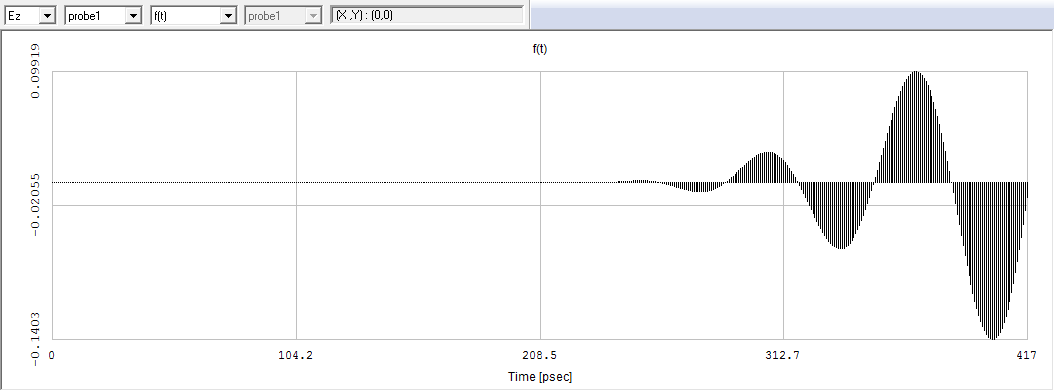
\includegraphics[width=0.95\linewidth]{graphics/35mm}
	}
	\subfigure[40 mm]
	{
		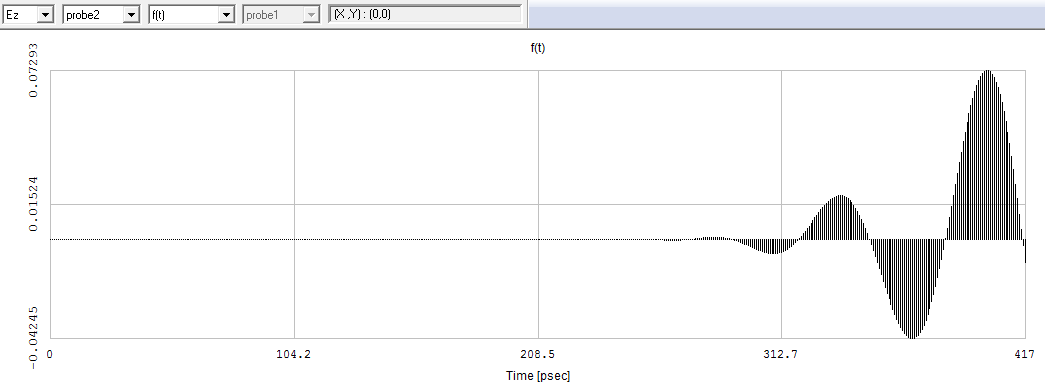
\includegraphics[width=0.95\linewidth]{graphics/40mm}
	}
	\caption{$E_z$ response at different distances from source}
	\label{fig:Task3-probes}
\end{figure}

Using the peak positive value for both probes with \eqref{eqn:alpha} gives:
\begin{equation*}
	\alpha = { \ln \left( { \SI{0.09919}{\volt\per\meter} \over \SI{0.07293}{\volt\per\meter} } \right) \over \SI{5}{\milli\meter}} = \SI{55.9}{\neper\per\meter}.
\end{equation*}
Using $\lambda = \SI{10}{mm}$ in \eqref{eqn:beta}:
\begin{equation*}
	\beta = {2 \pi \over \lambda} = \SI{628.31}{\radian\per\meter}.
\end{equation*}

\paragraph{Task 9} \textit{Compare the results of Task 8 to the theoretical values.}

The attenuation and phase constants are:
\begin{align*}
	\alpha &= { \omega \sqrt{\mu \epsilon} \over \sqrt{2} } \sqrt{\sqrt{1 + \left( {\sigma \over \omega \epsilon} \right)^2} - 1} \\
	&= { \omega \sqrt{\epsilon_r} \over c_0 \sqrt{2} } \sqrt{\sqrt{1 + \left( {\sigma \over \omega \epsilon_0 \epsilon_r} \right)^2} - 1} \\
	&= { 2 \pi \cdot \SI{15}{\giga\hertz} \cdot \sqrt{4} \over c_0 \sqrt{2} } \sqrt{\sqrt{1 + \left( {0.5 \over 2 \pi \cdot \SI{15}{\giga\hertz} \cdot \epsilon_0 \cdot 4} \right)^2} - 1} \\
	&= \SI{46.96}{\neper\per\meter}
\end{align*}
\begin{align*}
	\beta &= { \omega \sqrt{\mu \epsilon} \over \sqrt{2} } \sqrt{\sqrt{1 + \left( {\sigma \over \omega \epsilon} \right)^2} + 1} \\
	&= \SI{630.50}{\radian\per\meter}
\end{align*}

The numbers agree.

\paragraph{Task 10} \textit{Modify the waves in \texttt{Polarization\_TE.mef} to produce various kinds of polarizations}

\begin{figure}[htpb]
	\centering
	\subfigure[$A = 1,\: \phi_\Delta = \SI{0}{\degree}$]
	{
		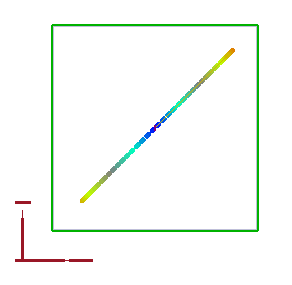
\includegraphics[width=0.475\linewidth]{graphics/Task4-lin}
		\label{fig:lin}
	}
	\subfigure[$A = 1,\: \phi_\Delta = \SI{-90}{\degree}$]
	{
		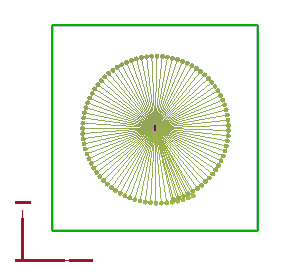
\includegraphics[width=0.475\linewidth]{graphics/Task4-RHC}
		\label{fig:RHC}
	}
	\subfigure[$A = 1,\: \phi_\Delta = \SI{45}{\degree}$]
	{
		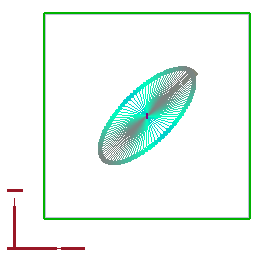
\includegraphics[width=0.475\linewidth]{graphics/Task4-LHE}
		\label{fig:LHE}
	}
	\caption{Various polarizations of a propagating electric field}
	\label{fig:polarization}
\end{figure}

Fig. \ref{fig:polarization} shows the result of changing $E_x$ and $E_y$. 

\section{Conclusion}\label{sec:conclusion}
The simulations in the lab vividly showed the electromagnetic theory that governs plane wave transmissions and reflections in a material at normal incidence.
It demonstrated how the waves behave in the first and second medium, especially the interactions of the incident wave and the reflected wave in the first medium. 

The simulation software can be used to check the calculations to see if the simulation and the calculation match up.
The reflection and transmission problems can be calculated using Smith charts. 

Electromagnetic transformers can be designed using the material properties and using materials with specific permittivity and adjusting the length of material sections to allow a specific amount of transmission. 


\newpage
\printbibliography[heading=bibintoc,title={References}]

\end{document}
